%---------------------Settings---------------------------%
\documentclass[10pt,a4paper,twocolumn,twoside,UTF8]{article}
\usepackage{geometry}
	\geometry{left=1.8cm,right=1.8cm,top=2.5cm,bottom=2cm}
% \usepackage{xeCJK}
\usepackage{amsmath,paralist,enumitem,booktabs,multirow,graphicx,subfig,setspace,listings,multicol,lettrine}
	\setlength{\parindent}{2em}
	\lstset{language=Python}
\usepackage{fancyhdr}
\usepackage{layout}
\setlength\columnsep{0.8cm}

%%begin----------Set header and footer----------------%%
\usepackage{ifthen}
\newboolean{first}
\setboolean{first}{true}
\pagestyle{fancy}
	\fancypagestyle{maincontent}{
		\fancyhf{}  
		\fancyhead[EL, OR]{\thepage}
		\fancyhead[EC]{C10 Application of Maximum likelihood estimate in signal separation}
		\fancyhead[OC]{GENERAL PHYSICS LABORATORY}
		\renewcommand\headrulewidth{0pt}
	}
	
	\usepackage{datetime}
	\fancypagestyle{firstpage}{
		\setboolean{first}{false}
		\fancyhf{}  
		\fancyhead[L]{Sun Yat-sen University}
		\fancyhead[R]{\shortmonthname[\the\month], \the\year}
		\fancyhead[C]{
		          \large{GENERAL PHYSICS LABORATORY}
		          }
	}
	
	\newcommand{\makefirstpageheadrule}{
	\makebox[0pt][s]{\rule[0.6\baselineskip]{\headwidth}{0.3pt}}
	\makebox[0pt][s]{\protect\hspace{-0.34em}\rule[0.75\baselineskip]{\headwidth}{0.3pt}}
	\protect\vspace{-20pt}
	}

	\newcommand{\makeheadrule}{
	\makebox[0pt][l]{\rule[1\baselineskip]{\headwidth}{0.3pt}}
	\protect\vspace{-20pt}
	}

	\renewcommand{\headrule}{
	\ifthenelse{\boolean{first}}{\makeheadrule}
	{\makefirstpageheadrule}
	}
%%end--------------Set header and footer-----------%%

%%begin-----------------Reference-----------------------%%
\usepackage[colorlinks,linkcolor=blue,urlcolor=blue,citecolor=blue]{hyperref}
\usepackage[hyperref=true,backend=biber,bibstyle=gb7714-2015,citestyle=numeric-comp,sorting=none,backref=true]{biblatex}
\addbibresource{REF.bib}
%%end-------------------Reference-----------------------%%

%end---------------------Settings---------------------------%




%%%%%%%%%%%%%%%%%%%%%%%%%%%%%%%%%%%%%%%%%%%%%%%%%%%%%%%%%%
%%%%%%%%%%%%%%%%%%%%%%%%%Document%%%%%%%%%%%%%%%%%%%%%%%%%
%%%%%%%%%%%%%%%%%%%%%%%%%%%%%%%%%%%%%%%%%%%%%%%%%%%%%%%%%%

%%begin-------------------Abstract-----------------------%%
\begin{document}
\title{\LARGE\textbf{Application of Maximum likelihood estimate in signal separation} \footnotemark[1]}
\author{\large\textit{Ziwei, Huang}$^{1}$\footnotemark[2]
\\ \normalsize{1 Zhongshan School of Medicine, Sun Yat-sen University, Guangzhou  { \rm 510275}, China}}
\date{}

\twocolumn[
	\begin{@twocolumnfalse}
	\maketitle  
	\renewcommand{\abstractname} {} 
	\begin{abstract}
	\vspace{-3em}
	{\bf Abstract: }
	{\small 
    Separating signals of interest from background noise is essential for identifying and classifying different events in particle physics experiments.
	To effectively separate the two types of events mixed in one observation, we employed a fully statistically based method called the maximum likelihood estimate, which appears to have a high classification performance. 
	A simulated observation containing two classes of normally distributed events was generated for demonstration. 
	Then, the maximum likelihood function was defined based on the observation, following which we minimized the maximum likelihood function to get the estimated parameters. 
	The result was further verified in the likelihood function space, and the confidence interval was calculated to evaluate the accuracy. 
	We also changed the proportion or the total number of events contained in the simulated observation, and repeated the process to probe into how the confidence interval responds to the properties of the observation. 
	We found that the maximum likelihood estimate is an effective framework for identifying and classifying different normally distributed events in a complex observation. 
	The confidence interval expends almost linearly as the total number of events increases, and the difference in confidence intervals of the two classes of events remains nearly consistent if the proportion remains consistent. 
	This study reveals the effectiveness of the maximum likelihood estimate in separating normally distributed events, providing a powerful tool for analyzing observation in particle physics experiments.
	}
	\par
	\textbf{Keywords: Maximum likelihood estimate, Particle physics experiment, Signal separation} 
	\vspace{2em}
	\end{abstract}
	\end{@twocolumnfalse}
]

\renewcommand{\thefootnote}{\fnsymbol{footnote}}
\footnotetext[1]{Supported and taught by Luyoutang, School of Physics, Sun Yat-sen University}
\footnotetext[2]{Corresponding author. ID: 20980066 Email: \url{huangzw29@mail2.sysu.edu.cn} }
%%end-------------------Abstract-----------------------%%

\thispagestyle{firstpage} 
\pagestyle{maincontent}

%%begin-------------------Intro-----------------------%%
\section{Introduction}

\lettrine[lines=2]{D}{ue} to some limitations of current commonly used particle signal detectors, the raw data obtained from a single observation may contain signals of many types of particle events.
For example, many detectors collect signals restricted in a specific energy interval, but it is quite common that many different types of particle event may share a similar characteristic energy level, e.g., solar neutrinos signals and radioactive decay signals.
This may lead to confusion when handling with these data.

To exclude the influence of background noise and get a specific type of signal of interest, it is essential to property classify these mixed events into different types. 
One robust approach is to take advantage of the characteristics of the statistic distribution of different types of events. 
Although signals of different classes of events may happen to have similar characteristic energy level, they may appear to show distinct statistic distributions. 
The determination of the classical model of statistic distribution of a certain type of event is knowledge-based, while the parameters are unknown. 
Previously, researchers might have to do this work manually according to their experience, but today with the aim of powerful computers, efficient algorithms can be applied to separate different signals accurately and automatically. 

In this work, we employed a fully statistically based method called a maximum likelihood estimate to separate different types of signal from a single observation, and the model achieved high classification performance.


%%end-------------------Intro-----------------------%%
% \newpage % Change the column
%%begin-----------------Method-----------------------%%
\section{Experimental principles and method}
	\subsection{Experimental principle\autocite{shenGeneralPhysicsLaboratory2015}}
		\subsubsection{Maximum likelihood estimate (MLE)}
		
		Maximum likelihood estimate, a fully statistical-based algorithm for parameters estimation based on frequency, 
		is an efficient method for classifying two types of events with different distribution patterns. 
		The core principle of this algorithm is to properly select a set of parameters $\theta^*$ to maximize the maximum likelihood function $L$, 
		which is defined as the probability of joint distribution of multiple samplings:
		\begin{gather}
			\theta^* = argmaxL(x_1, x_2, ..., x_n;\theta) \label{eq:1.1} \\
			L(x_1, x_2, ..., x_n;\theta) = \prod_{i=1}^n f(x_i;\theta) \label{eq:1.2}
		\end{gather}
		while $f(x_i;\theta)$ is defined as the probability density function.

		For example, assume that we have two types of normally distributed events, $A$ and $B$:
		\begin{align*}
			&A: f(x, \mu_1, \sigma_1) = \frac{1}{\sigma_1\sqrt{2\pi}}e^{{-\frac{(x-\mu_1)^2}{2\sigma_1^2}}} \\
			&B: f(x, \mu_2, \sigma_2) = \frac{2}{\sigma_2\sqrt{2\pi}}e^{{-\frac{(x-\mu_2)^2}{2\sigma_2^2}}}
			\label{eq:1.3}
		\end{align*}

		For a given energy interval, we can evenly divide the interval into small intervals $M$. 
		Then, for the $i$ th interval, we can calculate the number of events falling it. 
		We can always choose a large enough $M$ to promise that not too much events are included in every interval. 
		If this condition is satisfied, we can assume that the distribution of events in every interval conforms to Poisson distribution. 
		\begin{equation}
			\pi_i = \frac{\lambda_i^{k_i}e^{-\lambda_i}}{k_i!}
			\label{eq:1.4}
		\end{equation}
		when
		\begin{equation}
			\lambda_i = \sum_{j} \mu_j H_{ij}
			\label{eq:1.5}
		\end{equation}
		$\lambda_i$ is the expected number of events included in the $i$ th interval; $k_i$ is the actual number of events included in the $i$ th interval; 
		$H_{ij}$ is the normalization factor; $\mu_j$ is the expected number of events of type $j$ included in the interval $i$, $j=A,B$.

		Now, we can define the maximum likelihood function as:
		\begin{align}
			L(k,\lambda) &= \prod_{i=1}^n \pi_i \notag \\
						 &= \prod_{i=1}^n \frac{\lambda_i^{k_i}e^{-\lambda_i}}{k_i!}
			\label{eq:1.6}
		\end{align}

		To reduce computational complexity, we can take the logarithm of $L$: 
		\begin{equation}
			-lnL = \sum_{i} \lambda_i - k_i ln(\lambda_i)
 			\label{eq:1.7}
		\end{equation}

		Our goal is to estimate a suitable set of parameters $\theta^*$ to minimize $-lnL$. 
		This can be done using a lot of existing well-founded methods. 
		In our work, we chose to use the $scipy.optimize.minimize()$ method implanted in Python Scipy modules 
		(See \href{https://docs.scipy.org/doc/scipy-1.8.0/html-scipyorg/reference/generated/scipy.optimize.minimize.html}{scipy.optimize.minimize — SciPy v1.8.0 Manual}.

	\subsection{The confidence interval}
		To evaluate the performance and accuracy of the maximum likelihood estimate on signal separation, we calculated the confidence interval of the result. 
		When the total number of events is large enough, the distribution of the maximum likelihood function is similar to the $\chi^2$ distribution:
		\begin{equation}
			\chi^2 = -2ln\frac{\widetilde{L}(k;\mu_1,\mu_{i \neq 1}^*)}{L(k;\mu^*)}
			\label{eq:1.8}
		\end{equation}
		$L$ is the maximum distribution, while $\widetilde{L}$ is the distribution of other parameters when a specific parameter reaches its maximum distribution. 
		
		We have:
		\begin{align}
			\chi^2 &= 2(\widetilde{l}-l) = 2\Delta l \\
			l &= -lnL
			\label{eq:1.9}
		\end{align}

		To calculate the confidence interval, we can keep a specific parameter at its maximum distribution, 
		while changing other parameters one by one to obtain the $\mu_{l}$ and $\mu_h$ that satisfies the condition $\chi^2 = 1$, i.e. $\Delta l = 0.5$. 
		The confidence interval is defined as 
		\begin{equation}
			[\mu_{l}, \mu_{h}]
			\label{eq:1.10}
		\end{equation}	
		
		
	\subsection{Materials and instruments}
		\subsubsection{Data}
		For demonstration, we generated two sets of normally distributed signals and concatenated them into one sequence. 
		\begin{enumerate}[label=\arabic*.]
			\item Set $A$: 100 events; $\mu_1= 10MeV$; $\sigma_1 = 2MeV$
			\item Set $B$: 200 events; $\mu_2= 15MeV$; $\sigma_2 = 3MeV$
		\end{enumerate}

		To investigate how the confidence interval responds to the portion and total number of events of $A$ and $B$, 
		we also generated a sequence of data sets and repeated the process (Table \ref{tab:0.1} and Table \ref{tab:0.2}, details in the Supplementary information). 
		\begin{table}[htbp]
			\centering
				\begin{tabular}{ccc}
					\toprule
						        &Class A	&Class B    \\
					\midrule
					Data1  	&100	    &200	    \\					
					Data21	&150	    &200	    \\		
					Data22	&200	    &200	    \\			
					Data23	&250	    &200	    \\
					Data24	&300	    &200	    \\
					\bottomrule
				\end{tabular}
				\caption{\textbf{Change the proportion of the two events}}
				\label{tab:0.1}
		\end{table}

		\begin{table}[htbp]
			\centering
				\begin{tabular}{ccc}
					\toprule
						        &Class A	&Class B    \\
					\midrule
					Data31	&50 	    &100	    \\	
					Data32	&75 	    &150	    \\
					Data1  	&100	    &200	    \\					
					Data33	&125	    &250	    \\
					Data34	&150	    &300	    \\
					\bottomrule
				\end{tabular}
				\caption{\textbf{Change the total number of the two events}}
				\label{tab:0.2}
		\end{table}


		\subsubsection{Platform}
		The analysis was conducted in python (3.9.7). 
		The version of packages used in this study is described in detail in the supplemental information.

	\subsection{Method}
		\begin{enumerate}[label=\arabic*.]
			\item We first generated two classes of events according to the parameters described above and concatenated them into one sequence.
			\item Next, the maximum likelihood function $-lnL$ was defined based on the simulated data.
			\item Then, we used $minimize$ function in $Scipy$ to minimized the maximum likelihood function and obtained the maximum likelihood estimated parameters.
			\item Finally, the confidence interval was calculated to evaluate the accuracy.
		\end{enumerate}
%%end-------------------Method-----------------------%%

%%begin-------------------Result-----------------------%%
\section{Result}
	\subsection{Generation of the simulated data}
		$np.random.normal$ was used to generate two sets of simulated normally distributed events. 
		Fig. \ref{fig:1.1} shows the distribution of 100,000 class $A$ events and 100,000 class $B$ events, showing that they actually conform to the normal distribution.
		100 Class $A$ events and 200 Class $B$ events generated using the same model were then mixed to generate a simulated observation, which conformed the mixture normal distribution (Fig. \ref{fig:1.2}).
		\begin{figure}[htbp]
			\centering
			\subfloat[ ]{\label{fig:1.1}
			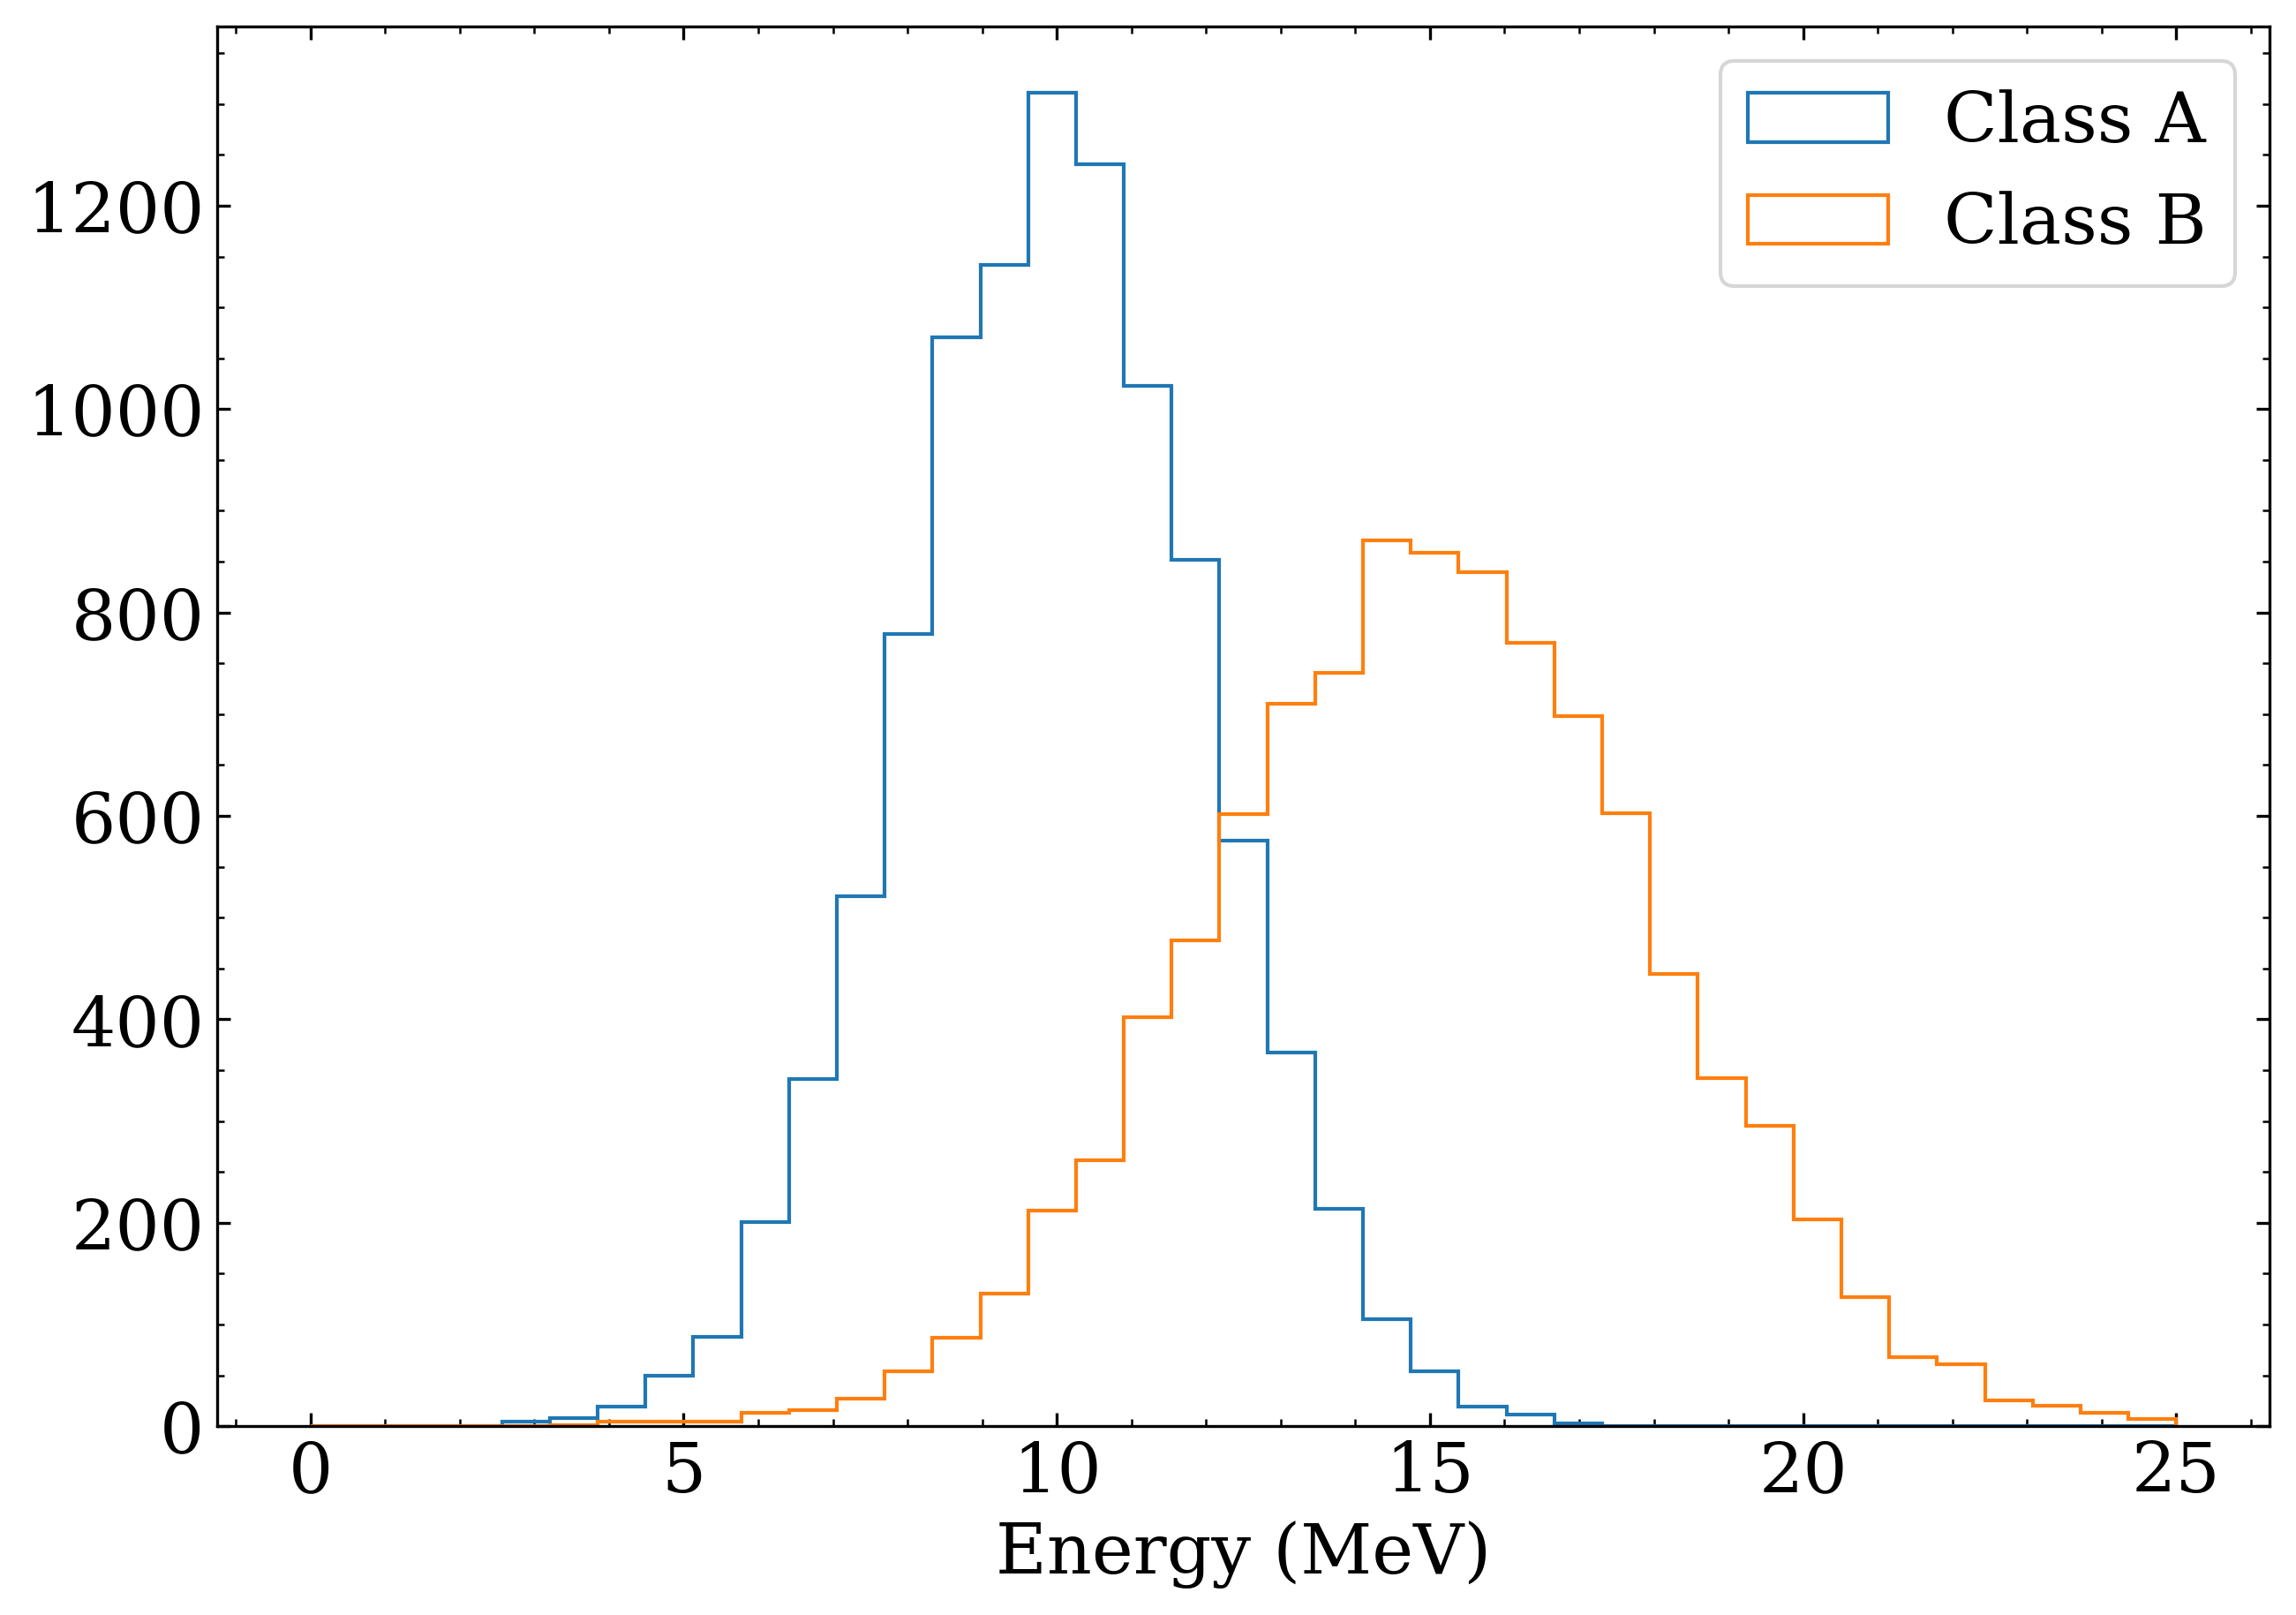
\includegraphics[width=0.24\textwidth]{attachments/fig.1.1.png}
			}
			\subfloat[ ]{\label{fig:1.2}
			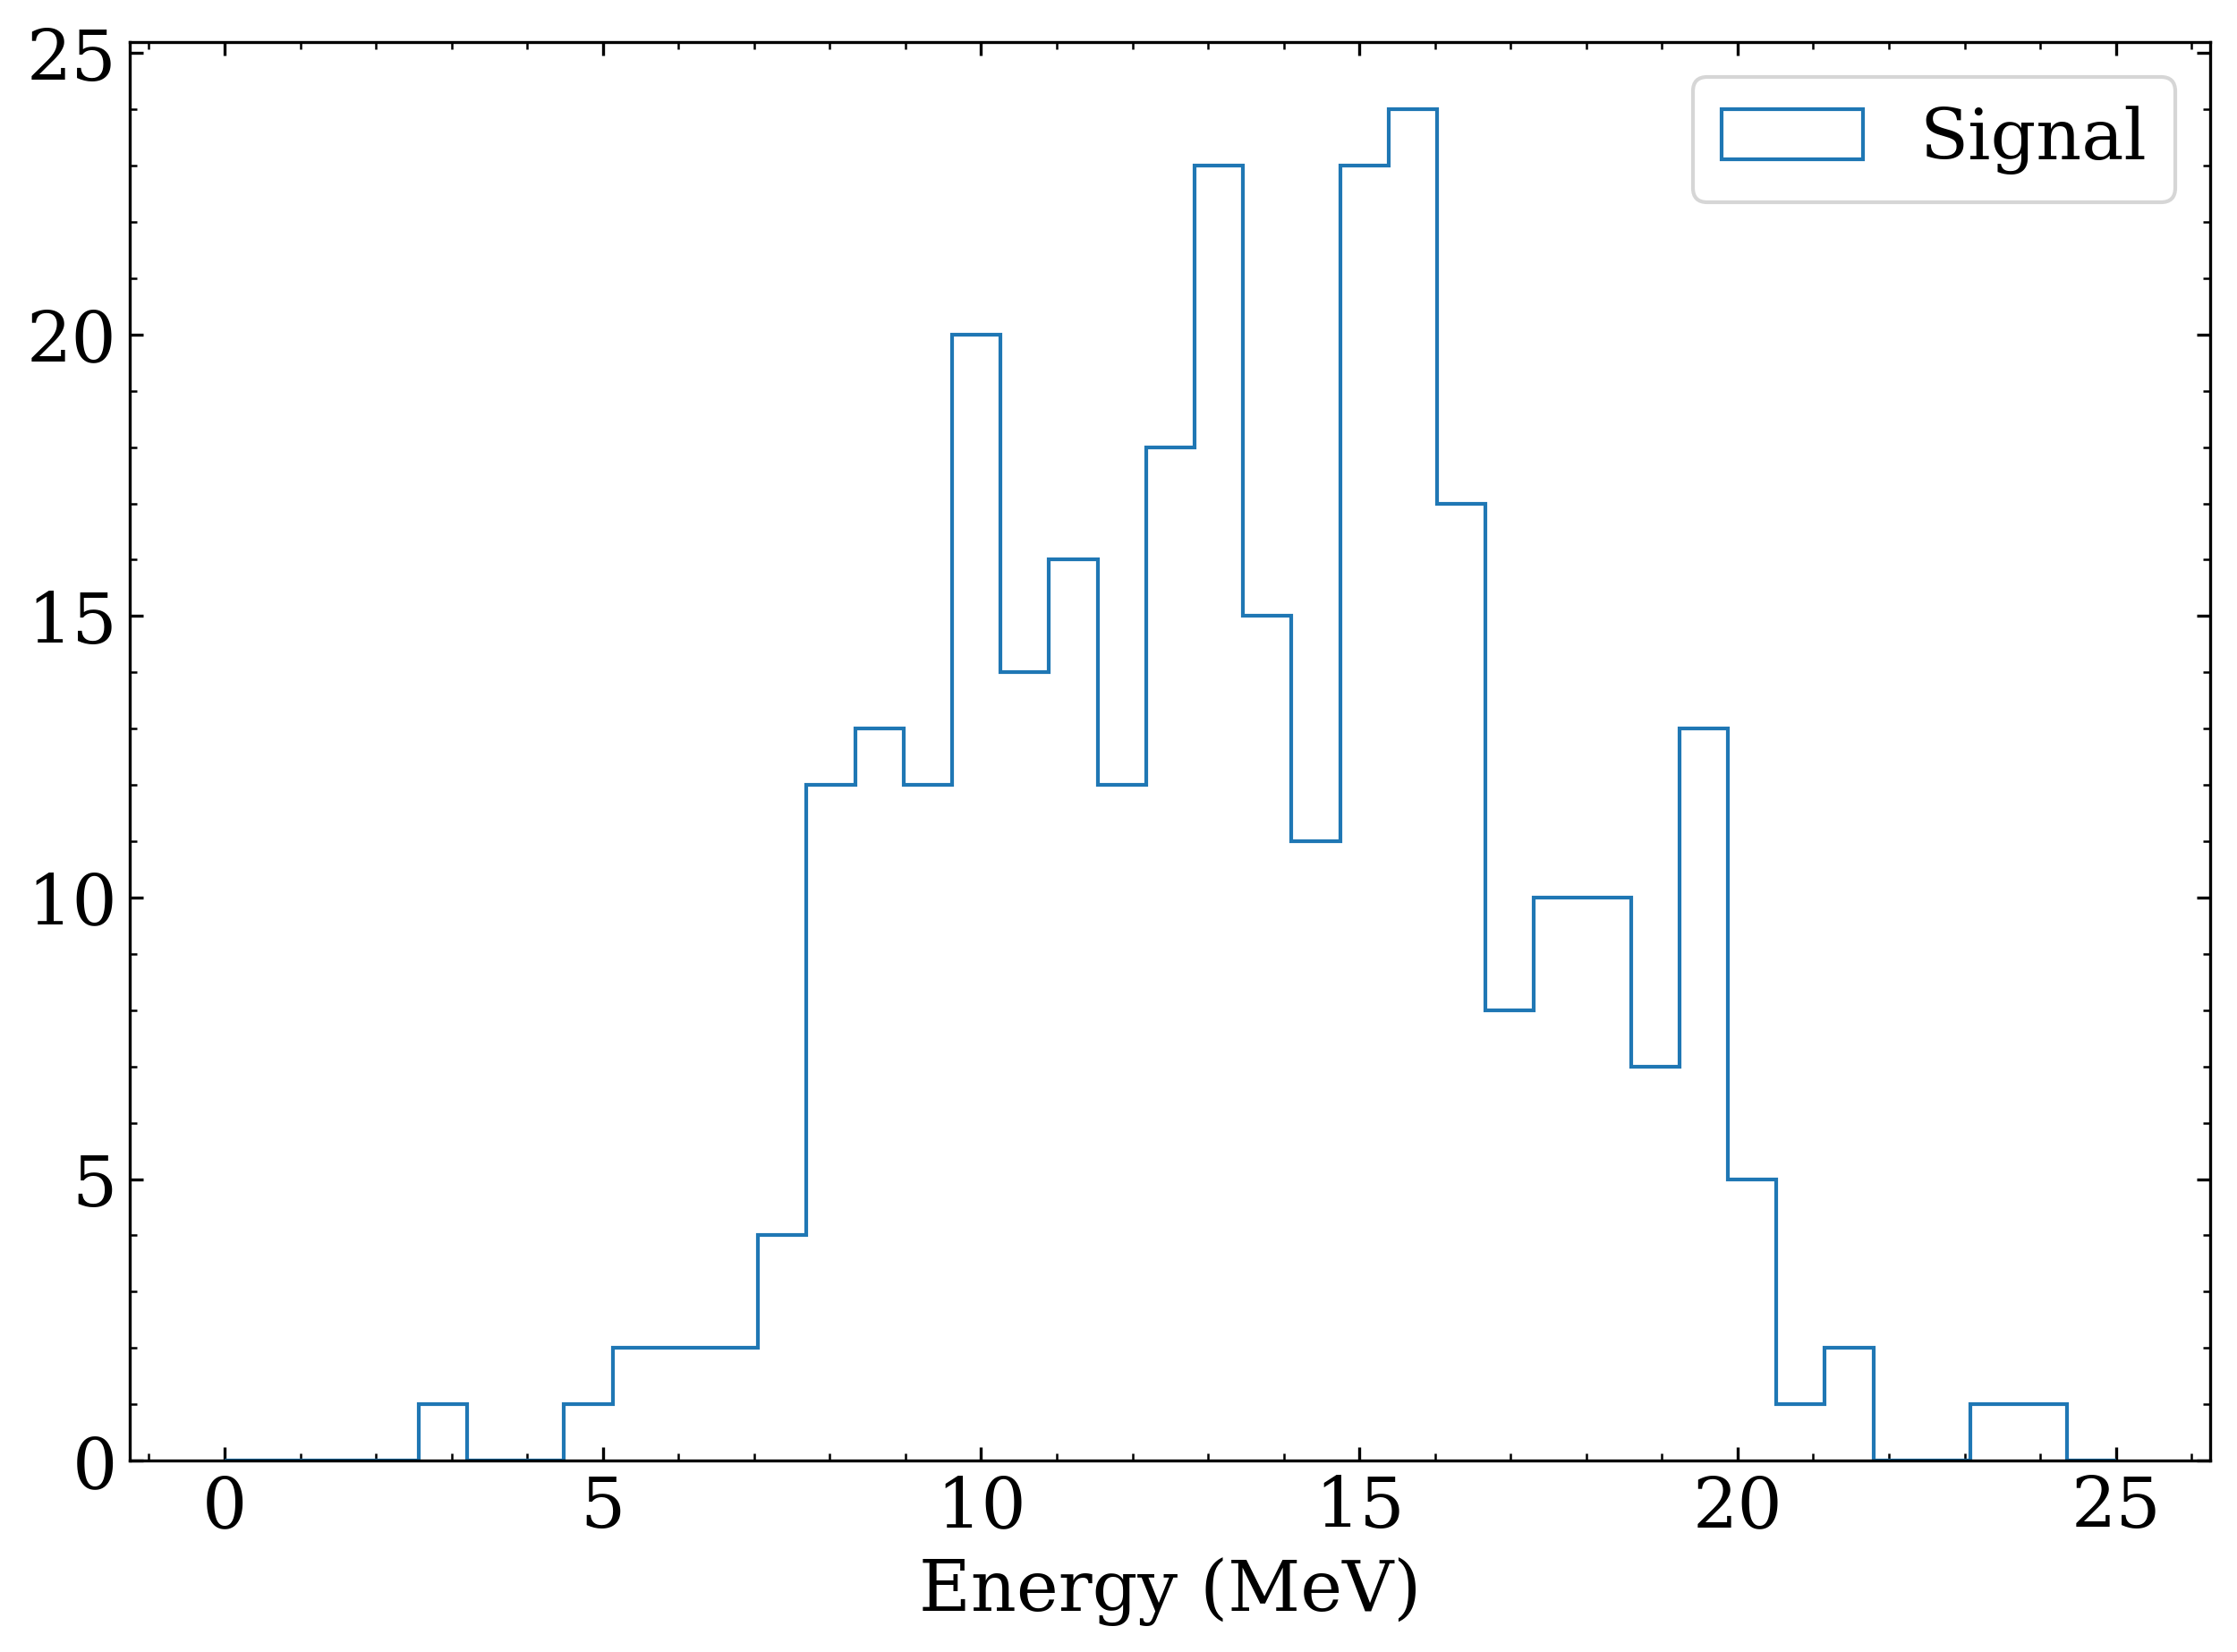
\includegraphics[width=0.24\textwidth]{attachments/fig.1.2.png}
			}
			\caption{\textbf{The distribution of the signals}}
		\end{figure}

	\section{Estimate the maximum likelihood parameters and fit the model}
		According to Equation \ref{eq:1.6}, the maximum likelihood function of the given data was initially defined. 
		To reduce the computational complexity, we further took the logarithm of $L$ (Equation \ref{eq:1.7}). 
		Then, the estimate parameters $\theta^*$ were calculated by minimizing the $-lnL$. 
		The results were verified in the likelihood function space (Fig. \ref{fig:2.1}). 
		\begin{figure}[htbp]
			\centering
			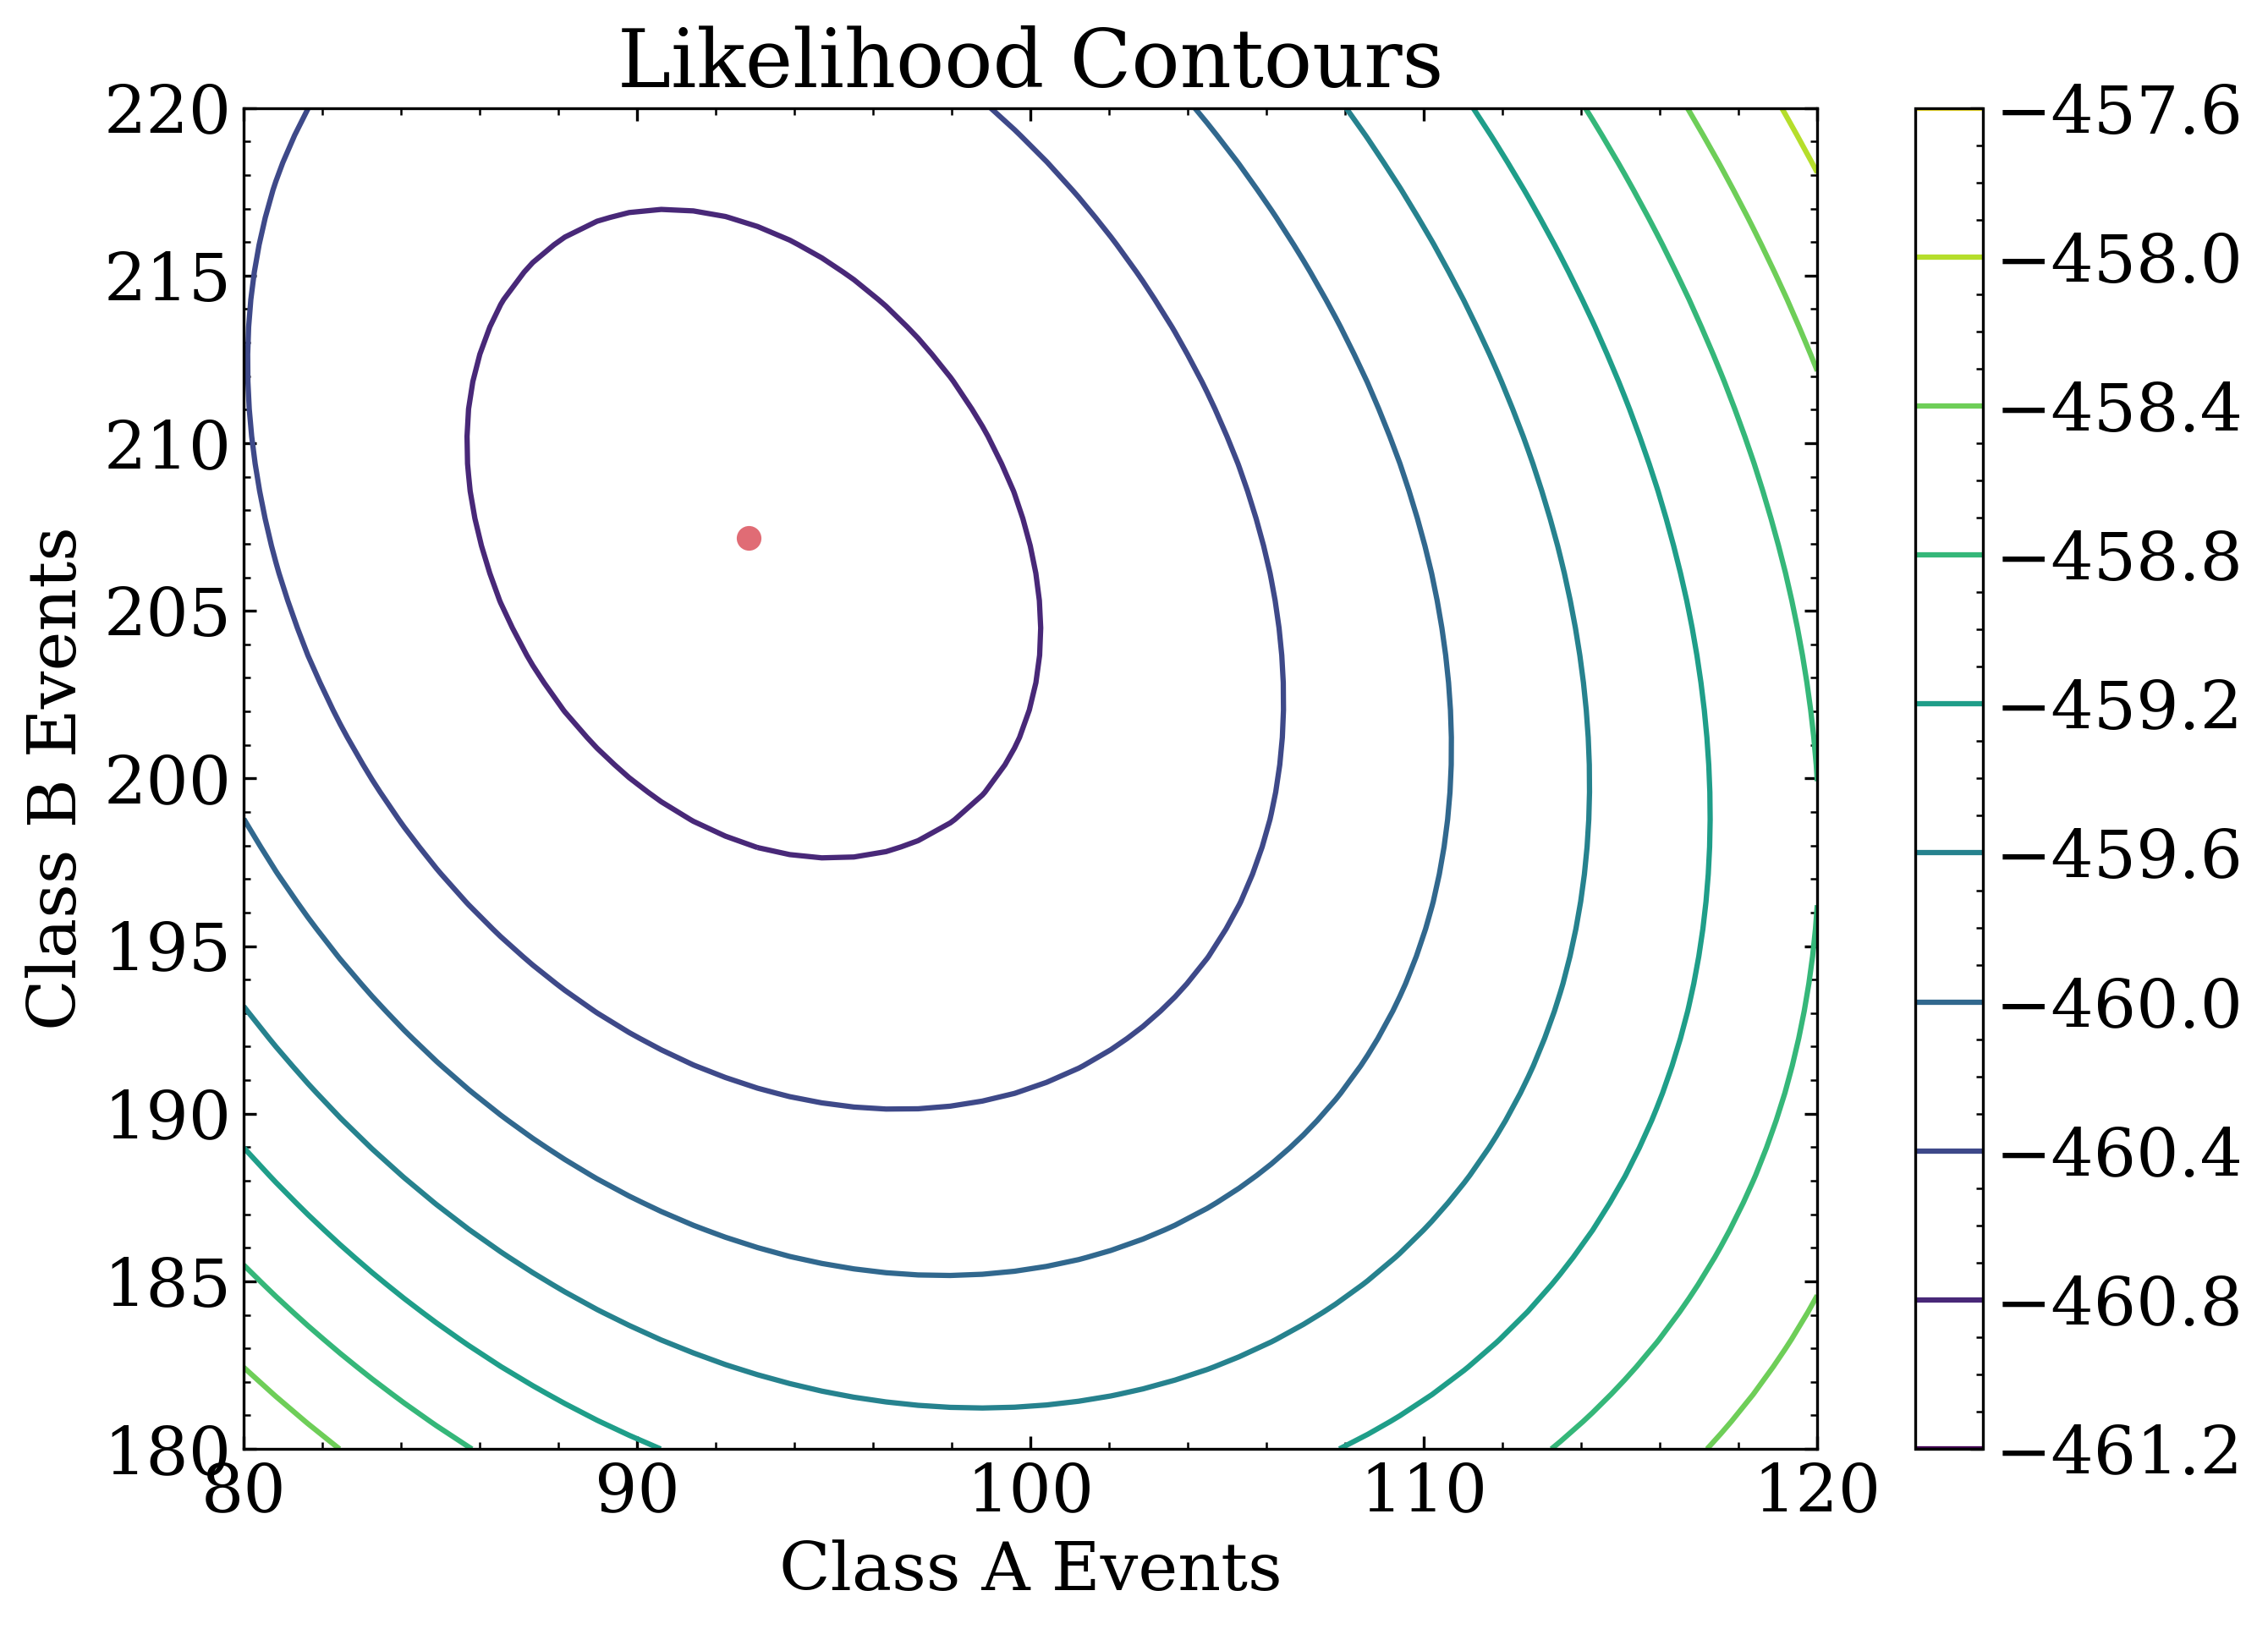
\includegraphics[width=0.4\textwidth]{attachments/fig.2.1.png}
			\caption{\textbf{Verify the results in the likelihood function space}}
			\label{fig:2.1}
		\end{figure}
	
		The resulting estimated parameters $\theta^*$ show a high consistency with our initial setting (Table \ref{tab:2.1}), 
		showing that the maximum likelihood estimate is an efficient method for separating two normally distributed signals.
		\begin{table}[htbp]
			\centering
				\begin{tabular}{ccc}
					\toprule
						        &Class A	&Class B    \\
					\midrule
					Setting	    &100	    &200	    \\
					Estimate	&92.837	    &207.163	\\
					\bottomrule
				\end{tabular}
				\caption{\textbf{Compare the estimate to the setting}}
				\label{tab:2.1}
		\end{table}

		Basing on the estimated parameters, the fitting signals of class $A$ and class $B$ together with the total fit 
		were generated and compared with the original observation (Fig. \ref{fig:2.3}). The performance of the model was satisfactory.
		\begin{figure}[htbp]
			\centering
			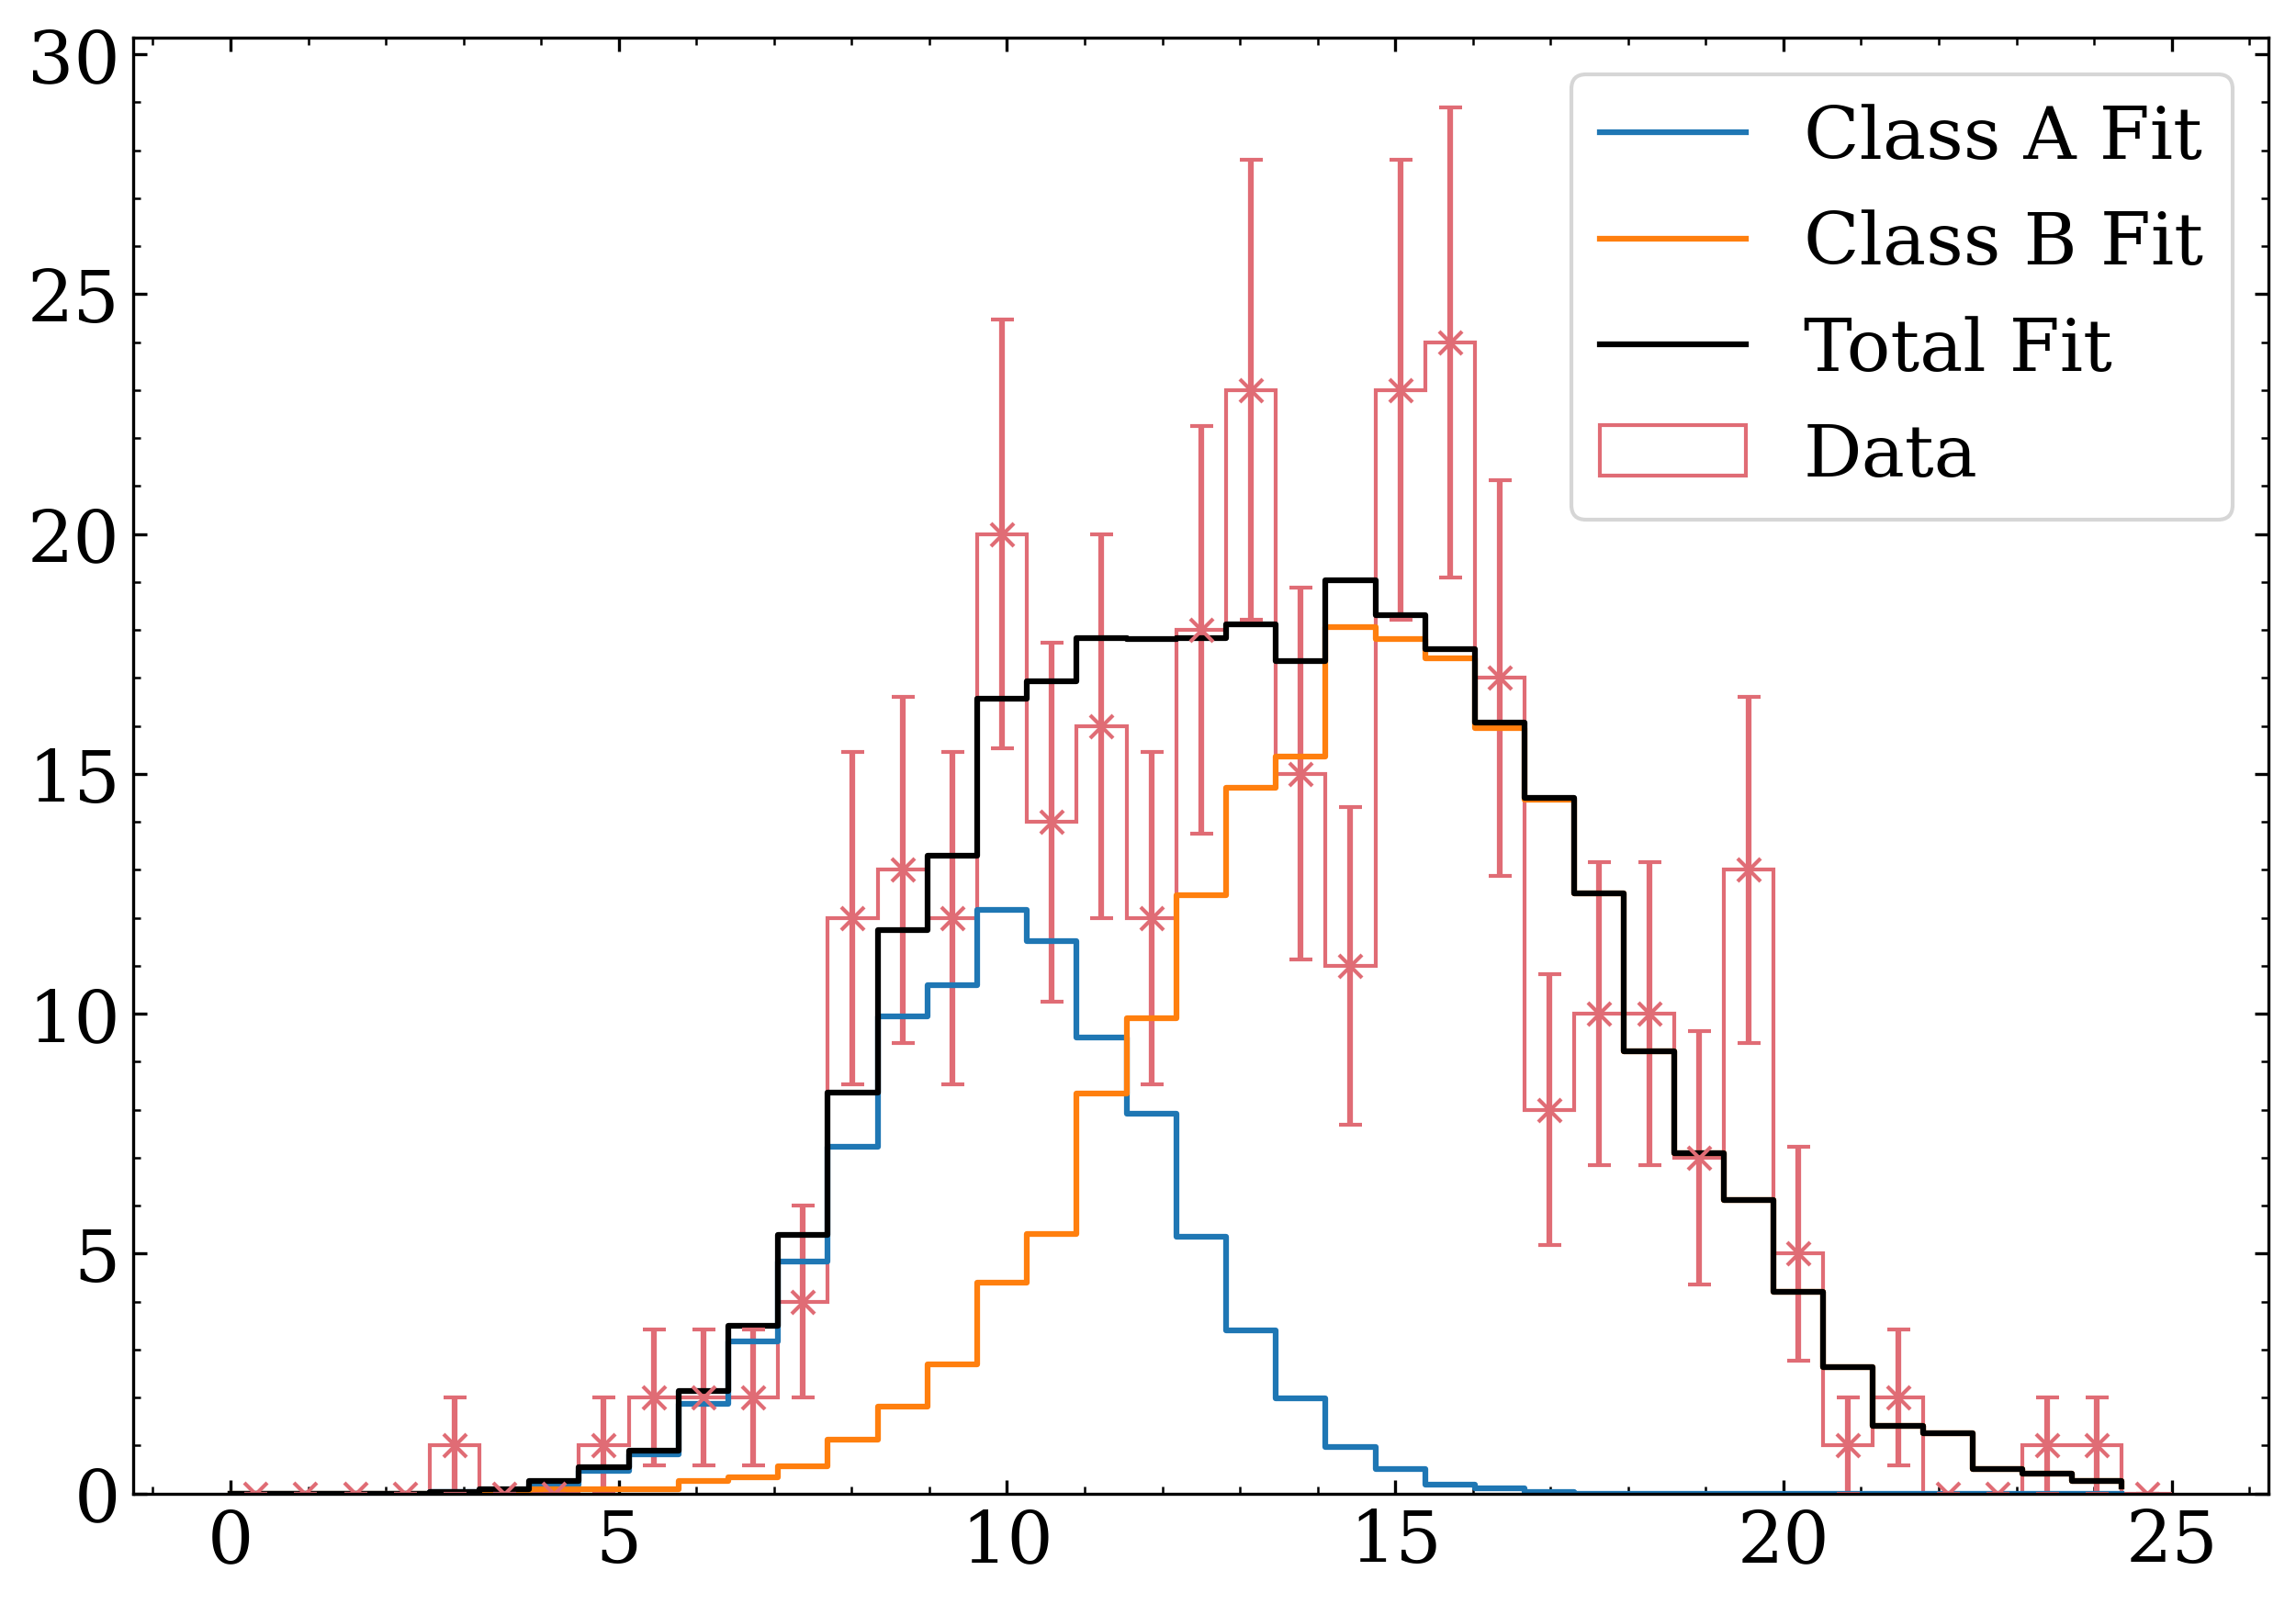
\includegraphics[width=0.4\textwidth]{attachments/fig.2.3.png}
			\caption{\textbf{Fitting the model}}
			\label{fig:2.3}
		\end{figure}

	\section{Calculate the confidence interval}
	To further evaluate the accuracy of the model, the confidence interval was calculated according to Equation \ref{eq:1.9}. 
	The profiles of the event $A$ and $B$ were plotted (Fig. \ref{fig:3.1}), and the confidence interval of the results are: 
	\paragraph{Class A} $92.84^{+12.63}_{-11.89}$
	\paragraph{Class B} $207.16^{+16.65}_{-15.88}$
	\begin{figure}[htbp]
		\centering
		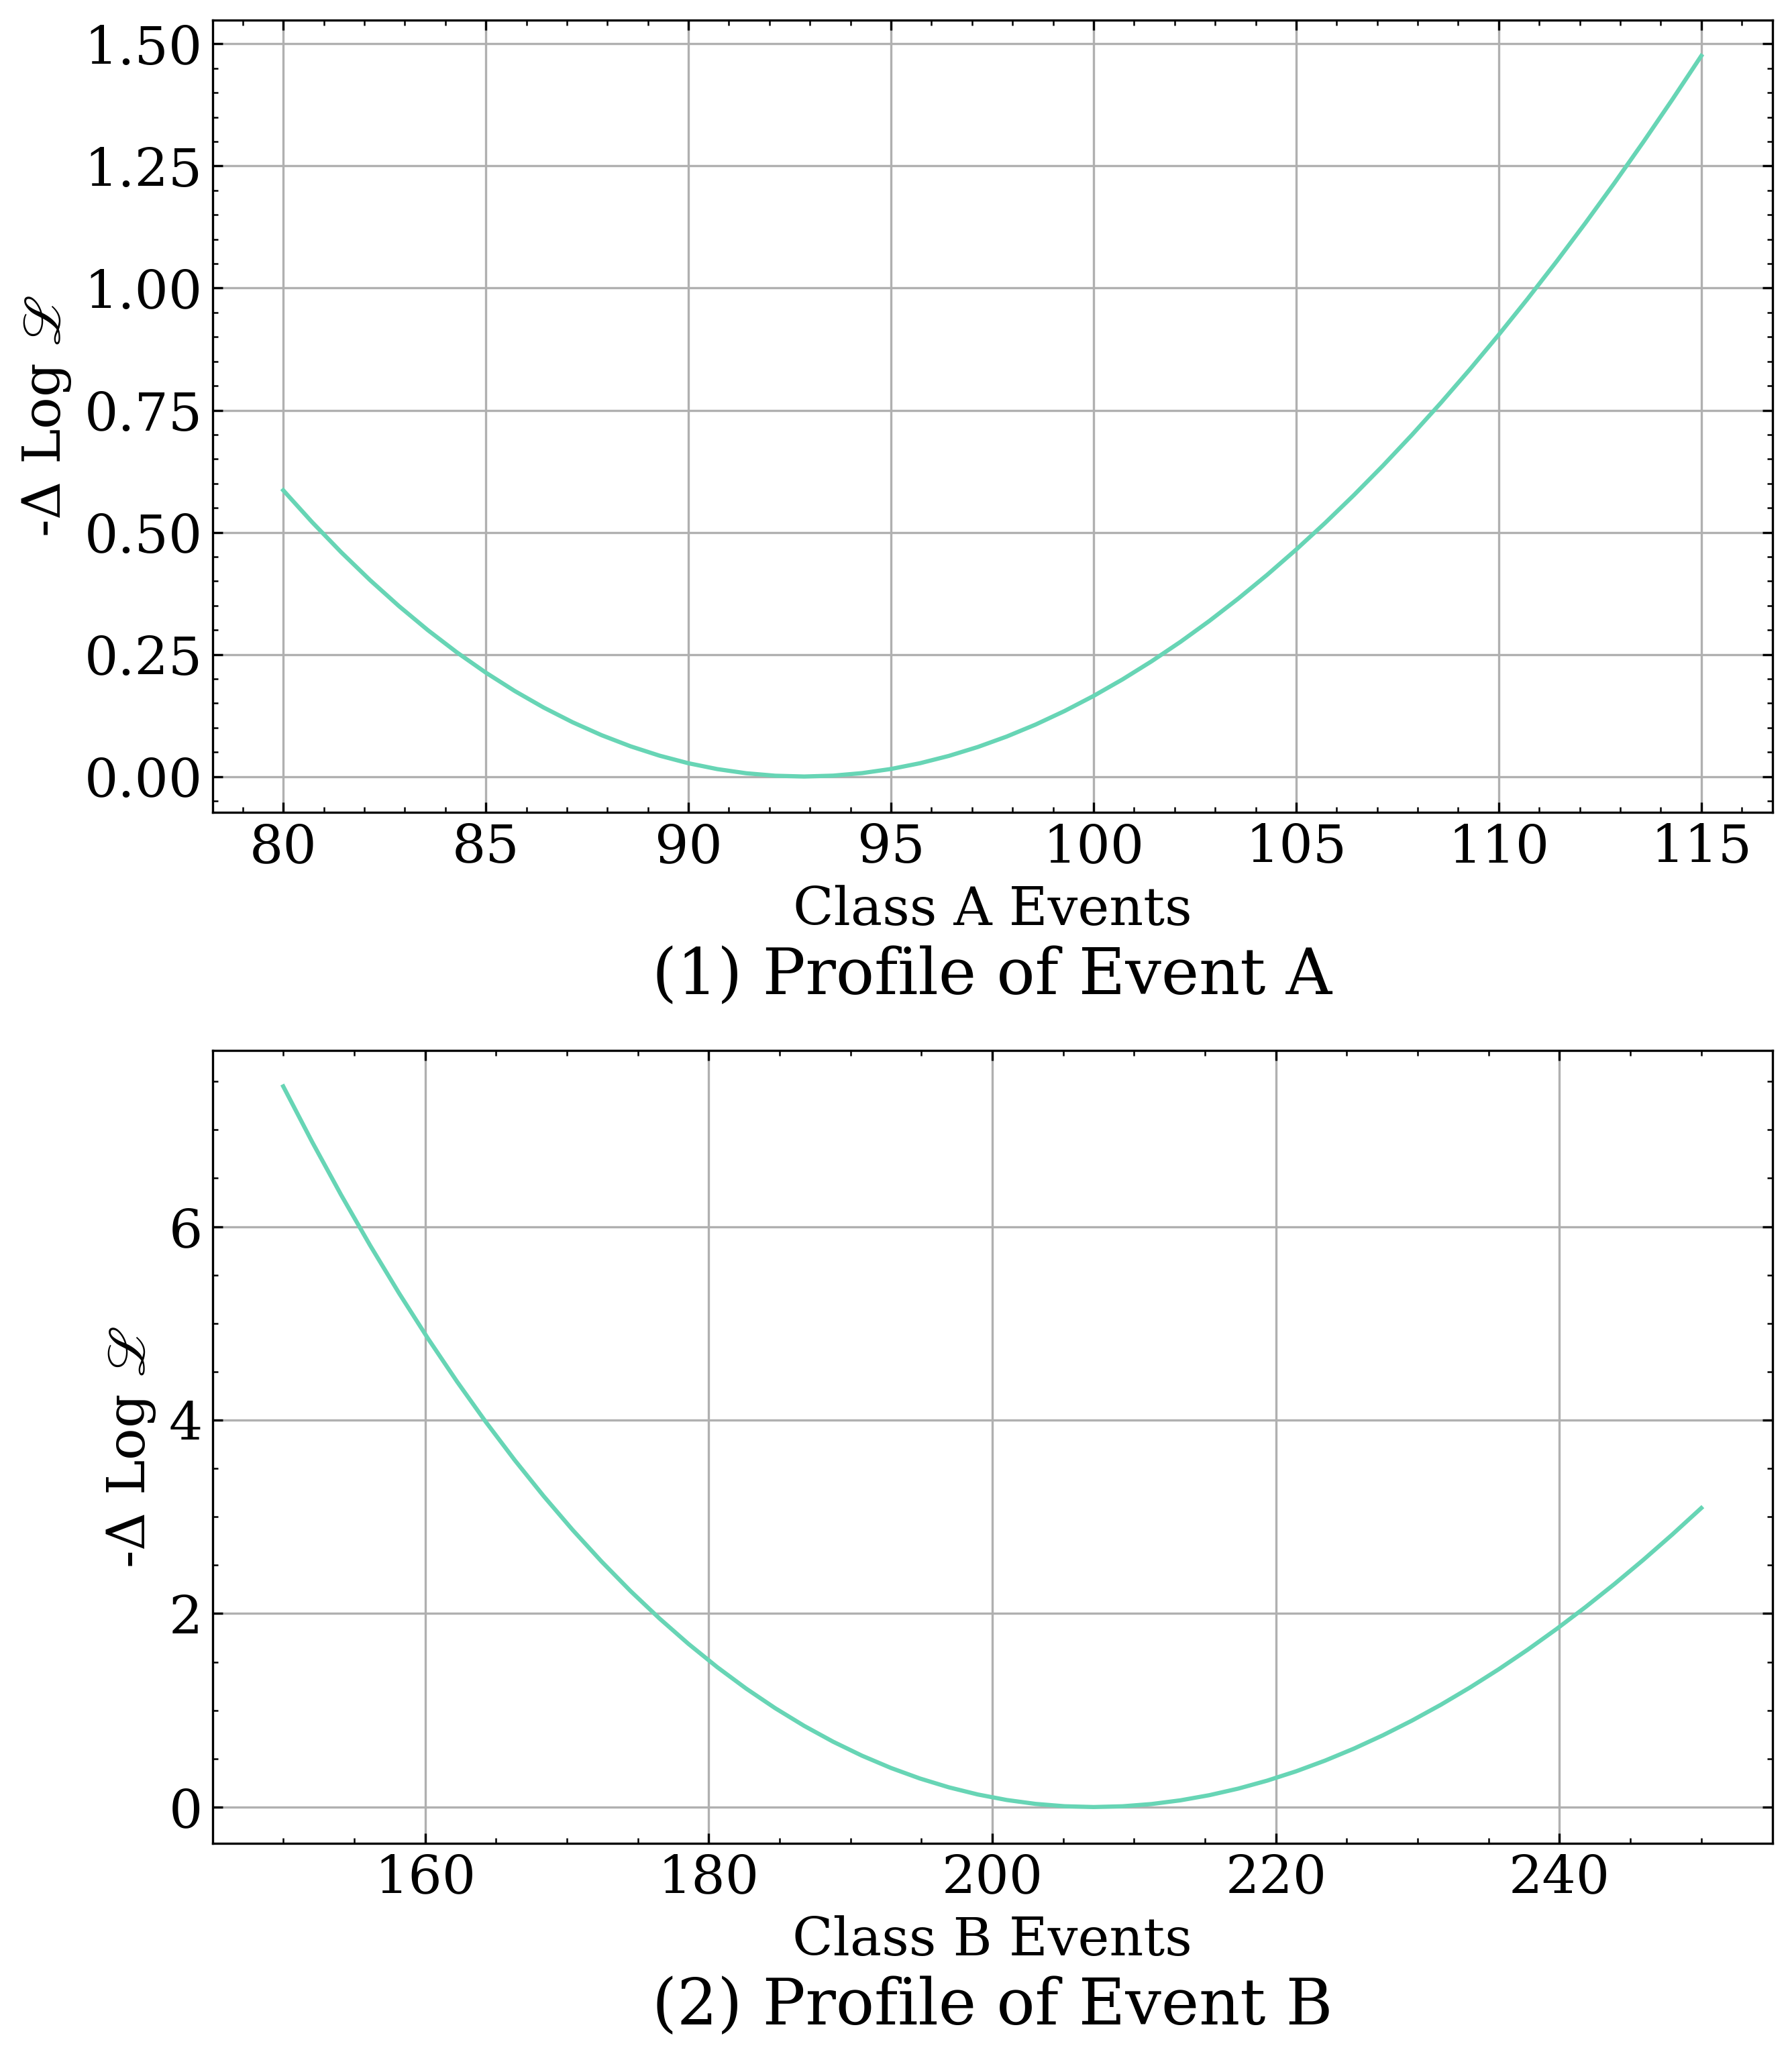
\includegraphics[width=0.4\textwidth]{attachments/fig.3.1.png}
		\caption{\textbf{Profiles of event A and B}}
		\label{fig:3.1}
	\end{figure}

	\section{Confidence interval responds to the properties of the observation}
	To probe into how the proportion and the total number of events in the observation affect the confidence interval, 
	we generated a series of observation (Table \ref{tab:0.1} and Table \ref{tab:0.2}) and test the confidence intervals. 
	The results show that the width of the confidence interval is perfectly positively correlated with the estimate number of the events 
	(Fig. \ref{fig:4.1}, $r_A=0.994$; and Fig. \ref{fig:4.2} $r_A=0.994$, $r_B=0.998$; See detailed regression parameters in the supplementary information)

	\begin{figure}[htbp]
		\centering
		\subfloat[ ]{\label{fig:4.1}
		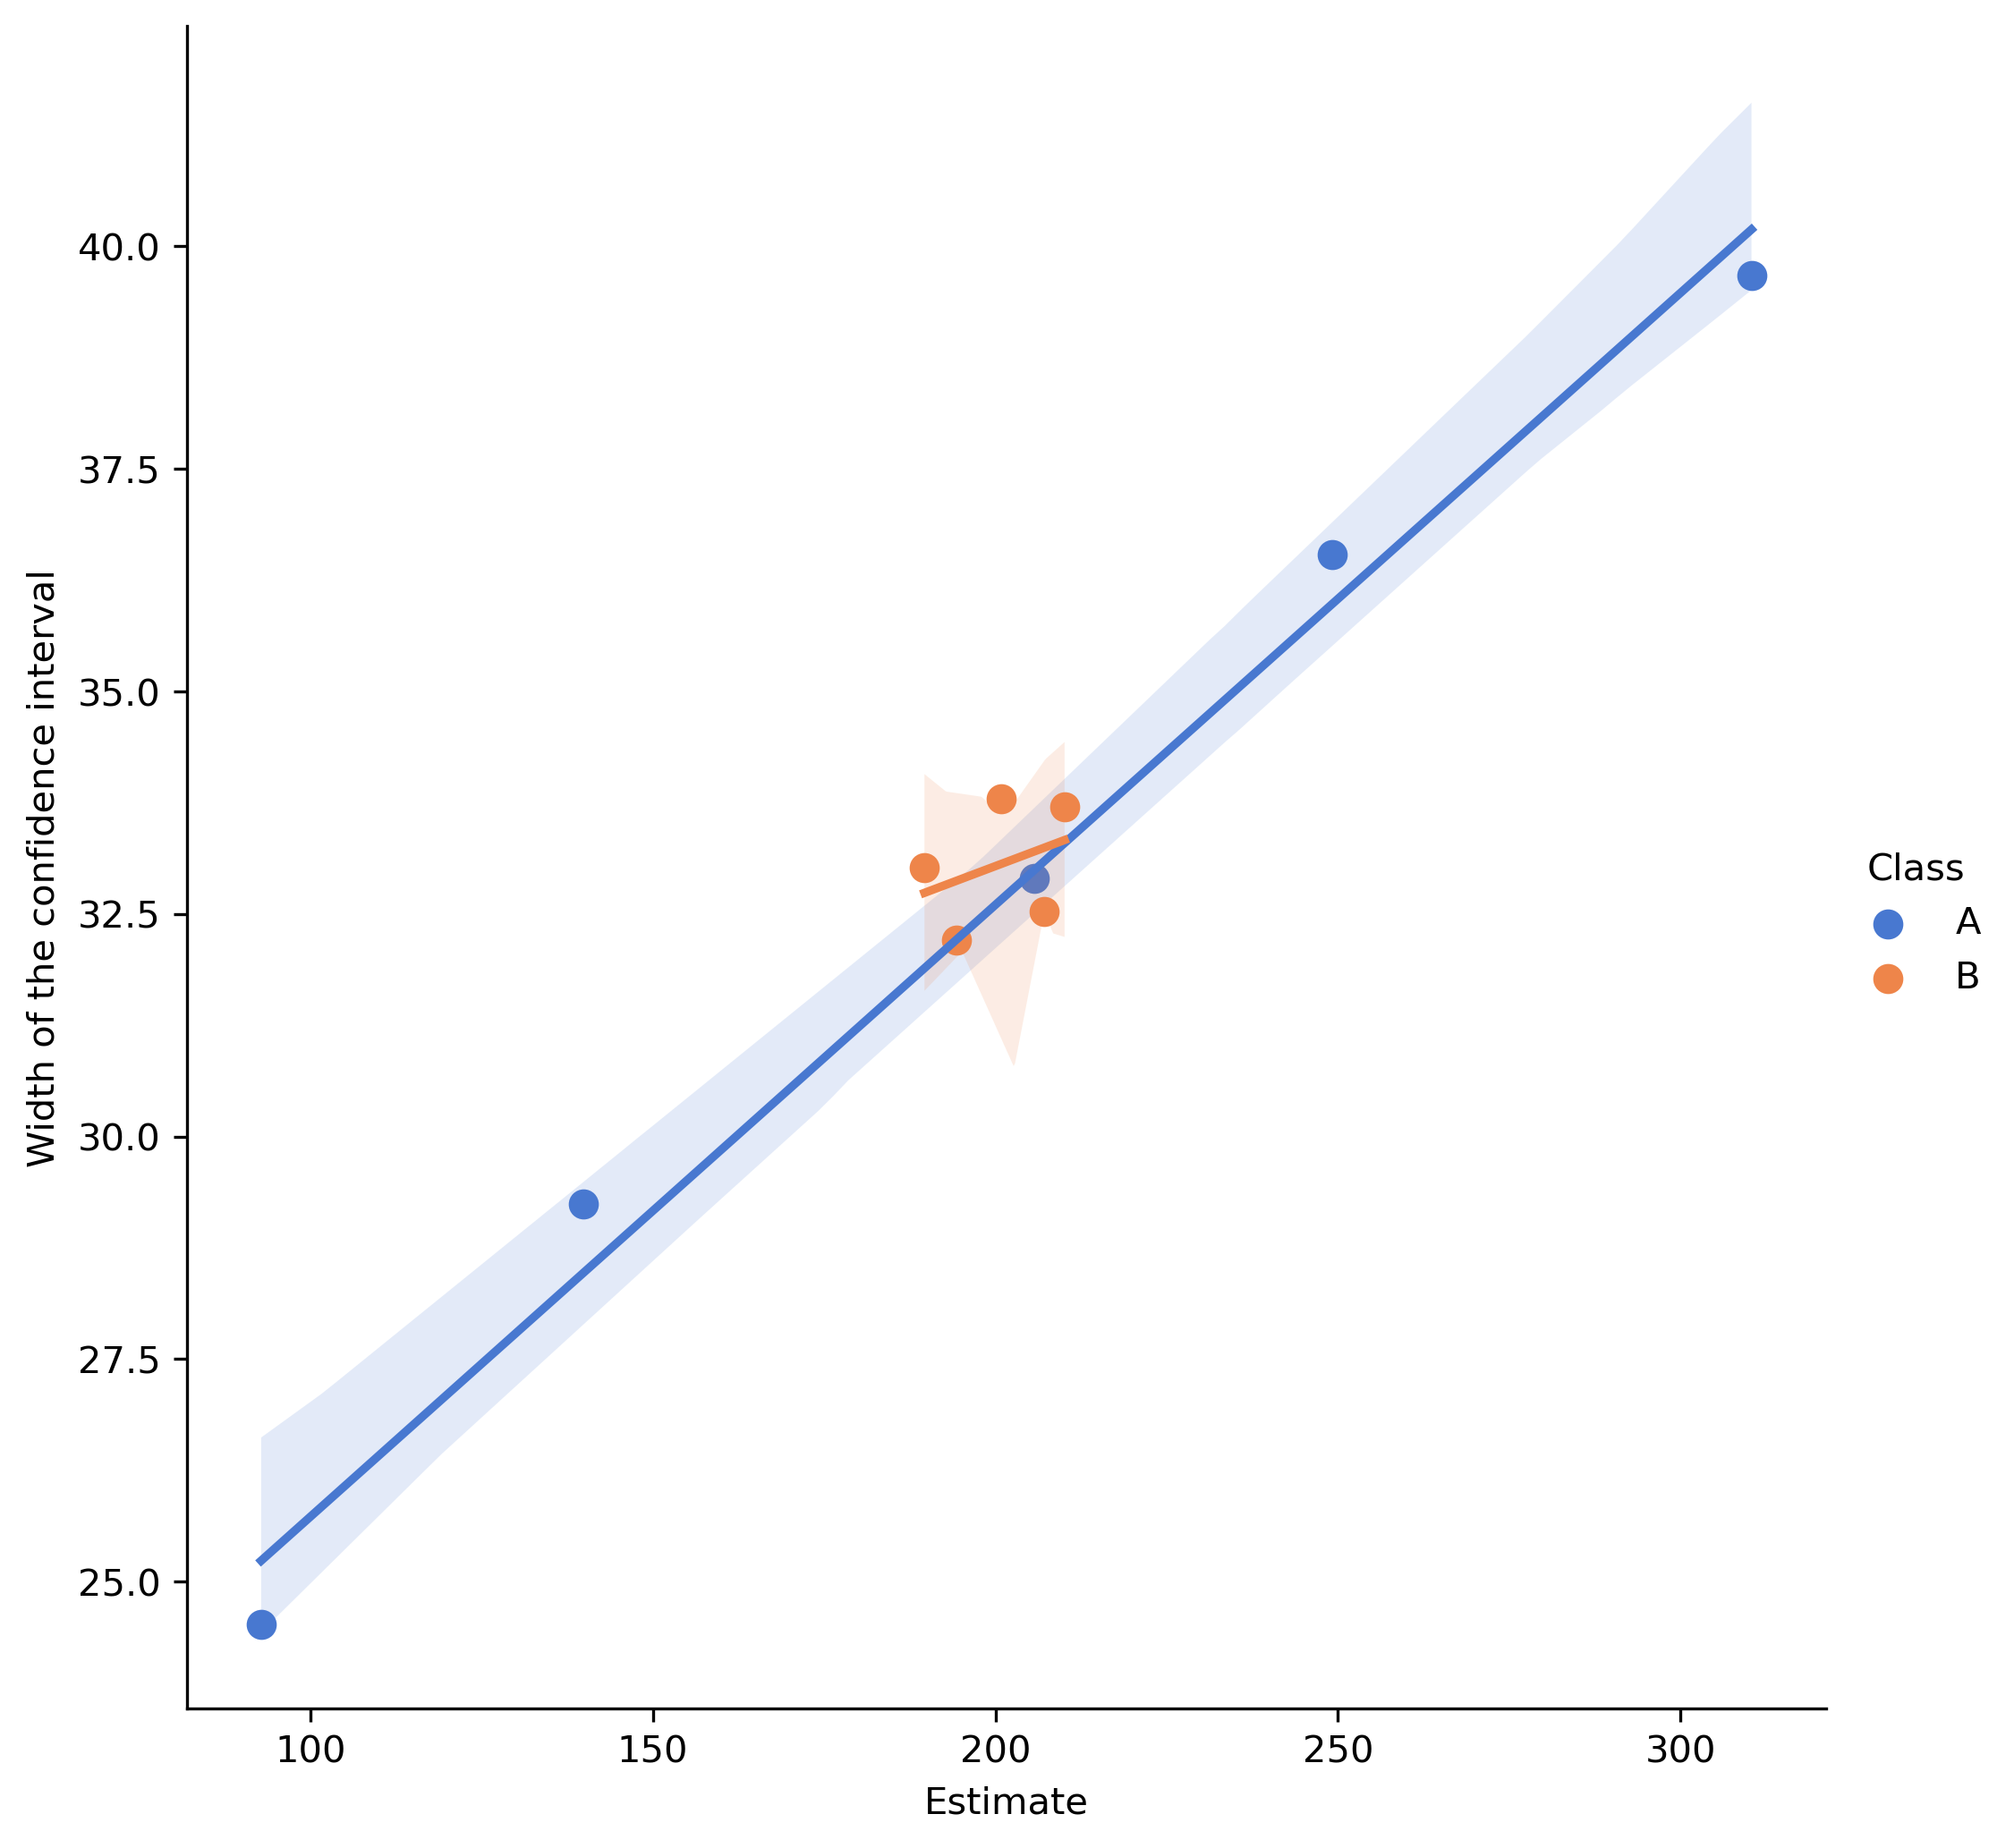
\includegraphics[width=0.24\textwidth]{attachments/fig.4.1.png}
		}
		\subfloat[ ]{\label{fig:4.2}
		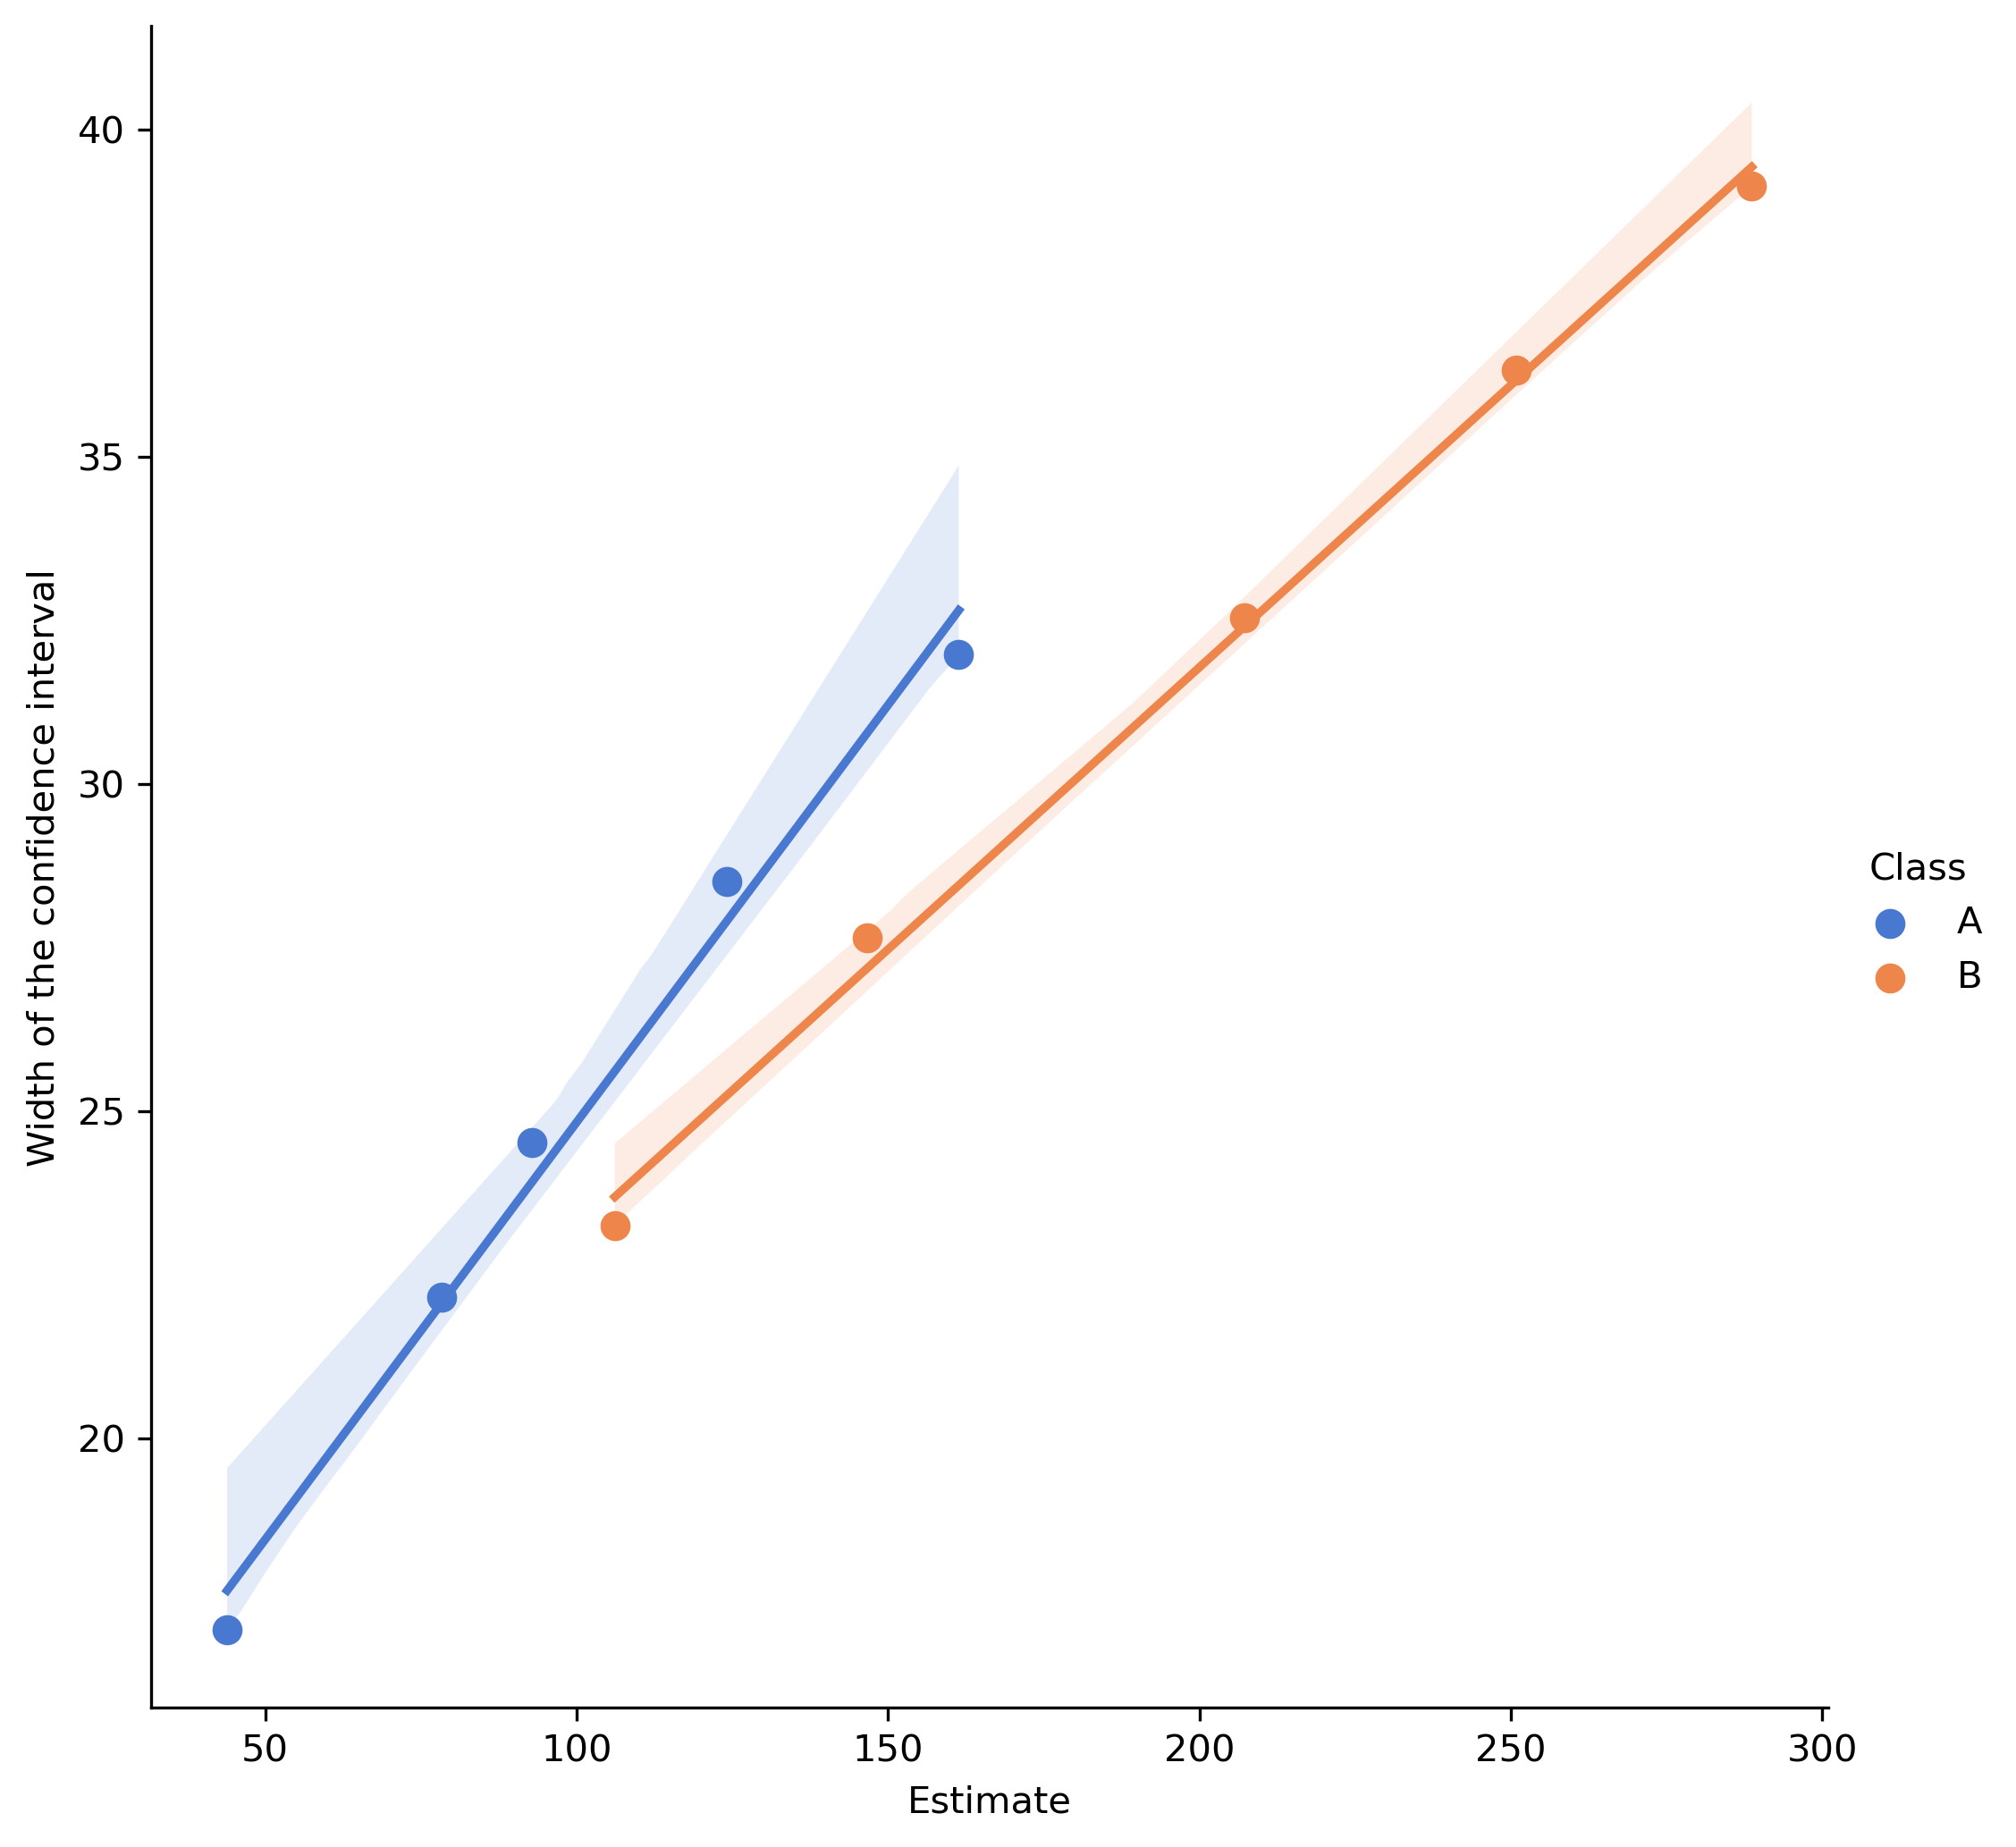
\includegraphics[width=0.24\textwidth]{attachments/fig.4.2.png}
		}
		\caption{\textbf{Confidence interval responds to proportion and the total number of the observation}}
	\end{figure}

%%end-------------------Result-----------------------%%

%%begin-------------------Conclusion and Discussion-----------------------%%
\section{Conclusion and Discussion}
	In this research we employed the maximum likelihood estimate on mixed observations and prove that it is an efficient algorithm to identify and classify different normally distributed events in a complex observation.
	We also found that the confidence interval expends almost linearly as the total number of events increases. 

		\subsubsection{Known limitation}
		However, there are still a few known limitations of this method when dealing with the real-world data:
		\begin{enumerate}[label=\arabic*.]
			\item In our experiment, we found that when the total number of events increases to about 1000, the algorithm becomes unstable and sometimes the maximum likelihood function cannot converge, which shows that the robustness of the algorithm should be further interrogated.
			\item As shown in the results, the width of the confidence interval expands almost linearly as the number of events increase, thus there is a consideration that whether the confidence interval is acceptable when dealing with real-world big data.
			\item In this experiment we only demonstrated separating two normally distributed signals from an observation using MLE, but whether this algorithm is compatible with signals conforming other distribution patterns is still unknown, which requires further research.
		\end{enumerate}


%%end-------------------Conclusion and Discussion-----------------------%%

%%end--------------------Reference------------------------%%
\printbibliography[title=Reference] 
%%end--------------------Reference------------------------%%
\end{document}